%************************************************
\chapter{Introduction to nucleic acid structure }\label{ch:introduction}
%************************************************
\section{Survey}
In Biology, organisms are living entities that consist of organs and the organs are made of tissues. The fundamental building blocks of the organisms that form tissues are cells. Cells consist of various molecules, and molecular biology is the field of science that studies cells at the molecular level. 

Molecules in the cell participate in various biochemical reactions to maintain the proper structure and function of the cell. Some micro-molecules are small molecules of low weights; they are often referred to as monomers. Many micro-molecules can join together to form more complex molecules called macromolecules. There are four essential macromolecules in the cell: the nucleic acids, the lipids, the proteins and the carbohydrates. Nucleic acids carry the genetic blueprint and the instructions for the functioning of the cell. Lipids include fats, waxes, oils, hormones, and specific components of membranes and function as energy-storage molecules and chemical messengers. Proteins are one of the most abundant organic molecules in the living systems; they contribute to many functional activities: enzymatic catalyses, contractility, formation of selectively permeable membranes, reversible binding and transport, and immunological activities. Finally, carbohydrates are an essential part of our diet. They provide energy to the body; grains, fruits and vegetables are all considered natural sources of carbohydrates.

Our work focuses on nucleic acids. The nucleic acids are made up of small repetitive micro-molecules called nucleotides. Genetic information necessary to specify the proteins needed by the organisms is contained in a nucleic acid called deoxyribonucleic acid (DNA) or, in some cases, for some viruses in the ribonucleic acid (RNA). This introductory chapter of the thesis presents a brief overview of the two types of nucleic acids, emphasising a particular class of RNAs (the non-coding RNAs). The overview concepts contain biological concepts and biochemical structure definitions of the non-coding RNAs. Although each overviewing concept has its origin and sometimes forms a separate discipline, they contribute to creating the basis and understanding of computational methods and different results presented in this thesis.  

\section{Deoxy-nucleic Acids (DNAs)}
DNAs are macromolecules in the nucleus of eukaryotic cells that allow storing information with the help of nucleotides. Nucleotides consist of a five-carbon sugar, a phosphate group, and a nucleobase. There are four nucleotides in the DNA, distinguished by their nucleobase: A for Adenine, T for Thymine, G for Guanine, and C for Cytosine. Even though the basis blocks constituting the DNA were known for many years, in 1953, James Watson and Francis Crick \cite{watson1953molecular} succeeded in putting them together and suggested a reasonable DNA structure. Their work counted on DNA X-ray diffraction patterns produced by Rosalind Franklin and Maurice Wilking and the data from Erwin Charganp. This work revealed for the first time that the structure of DNA molecules has helical chains, each coiled around the same axis where the chain consists of phosphate dieter groups. The two chains are held together by the purimide and pyrimidine bases; they are joined together in pairs, a single base from the other chain bonded to a single base from the other chain. For the bounding to occur, one of the pairs must be Adenine and thymine or Guanine and Cytosine. The complementary pairing of the bases was then compatible with Chargaff's empirical rules---the amount of pyrimidine nucleotides (T+C) always equals the total number of purine nucleotides (A+G). 
\graffito{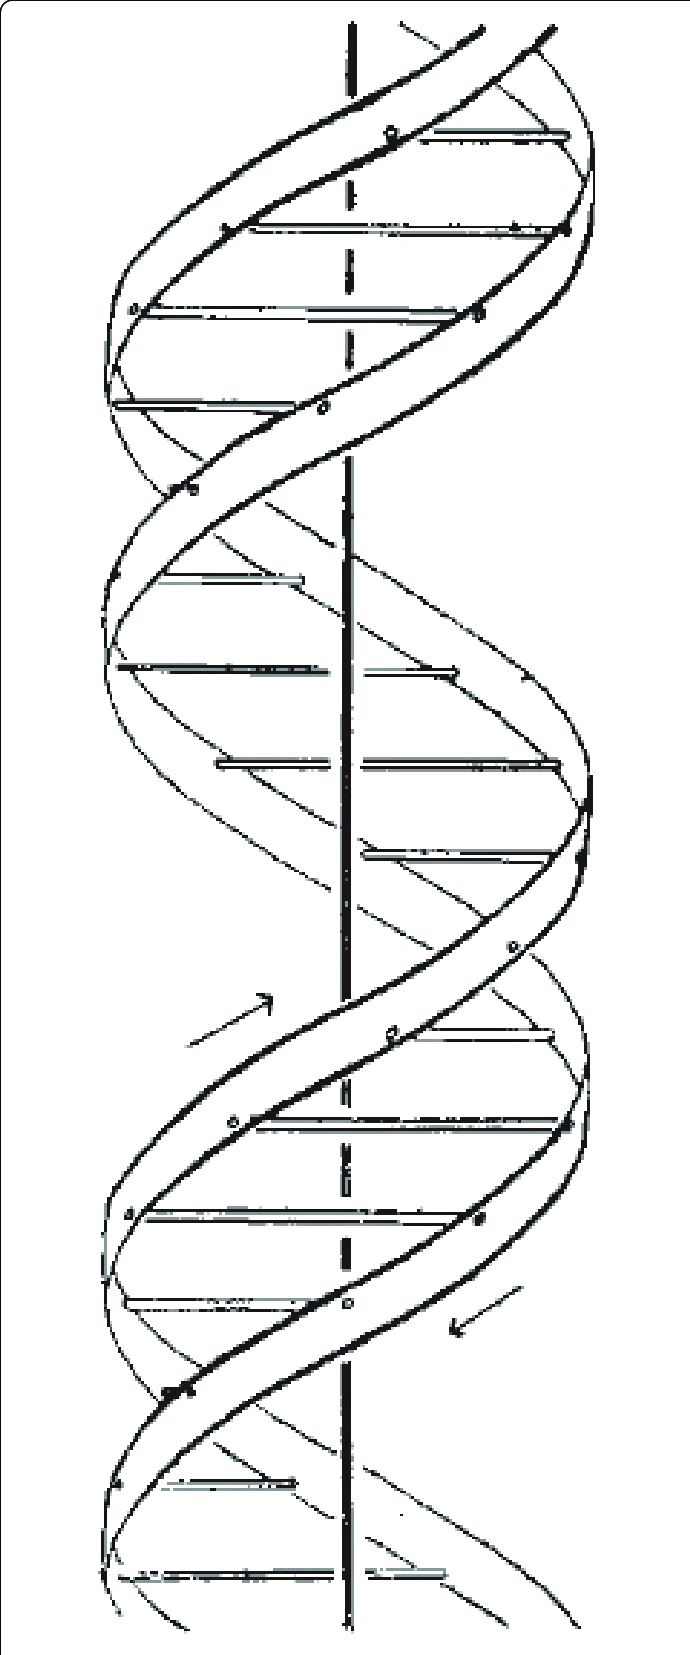
\includegraphics[width=1\linewidth]{../res/images/dna.png}
		Helical representation of DNA structures \cite{watson1953molecular}.}

Watson and Crick's elucidation of DNA structure has motivated many other scientists for further investigations and gave rise to modern molecular biology. Later in the same year, Watson and Crick formulated the central dogma of molecular biology that describes the flow of information between DNA, RNA, and proteins. They described the dogma in two steps: from DNA to mRNA through transcription and from mRNAs to proteins through translation. Since this central dogma was proposed, more works have been done to investigate each step. DNAs are transcribed into RNA molecules (messenger RNAs) that contain the same information as the template DNAs. Subsequently, these RNA messengers are translated into proteins according to the genetic code [Miller et al., 2009]. 
Several works also revealed that DNAs could perform some catalytic reactions. Still, the implication of RNAs in most vital chemical reactions in living systems and its broader range of chemical reactions have motivated many scientists in the last decay to study RNA molecules in more detail as an independent entity. The next section of our work focuses on the biochemistry of RNA structure in general, especially highlighting the biological importance of non-coding RNAs. 

\section{non-coding RNAs and their biological implications} 

So far in this work, RNAs have been mentioned only in the context of the central dogma of microbiology. That may imply that RNAs play the same typical role as DNAs, which is the genetic information memory. But not all RNAs are translated into proteins; in other terms, not all RNAs are mRNAs. There are mainly two RNA groups: coding RNAs (cRNAs) translated into proteins and non-coding RNAs that are not translated into proteins. In the previous section, we introduced the central dogma of microbiology, which describes the flow of information in the living systems. In other terms, data flows from nucleic acids to proteins and not vice versa. During the transcription and the translation steps in the information flow, there are some vital functions performed by non-coding RNAs such as ribosomal RNA (rRNAs) and transfer RNAs (tRNAs). The study of such RNAs revealed that rRNAs, rather than ribosomal proteins, catalyze the synthesis of proteins (i.e. the polymerization of amino acids), distinguish between correct and incorrect codon-anticodon pairs and prevent the premature hydrolysis of peptidyl-tRNAs \cite{moore2011roles, breaker2006rna}.
\graffito{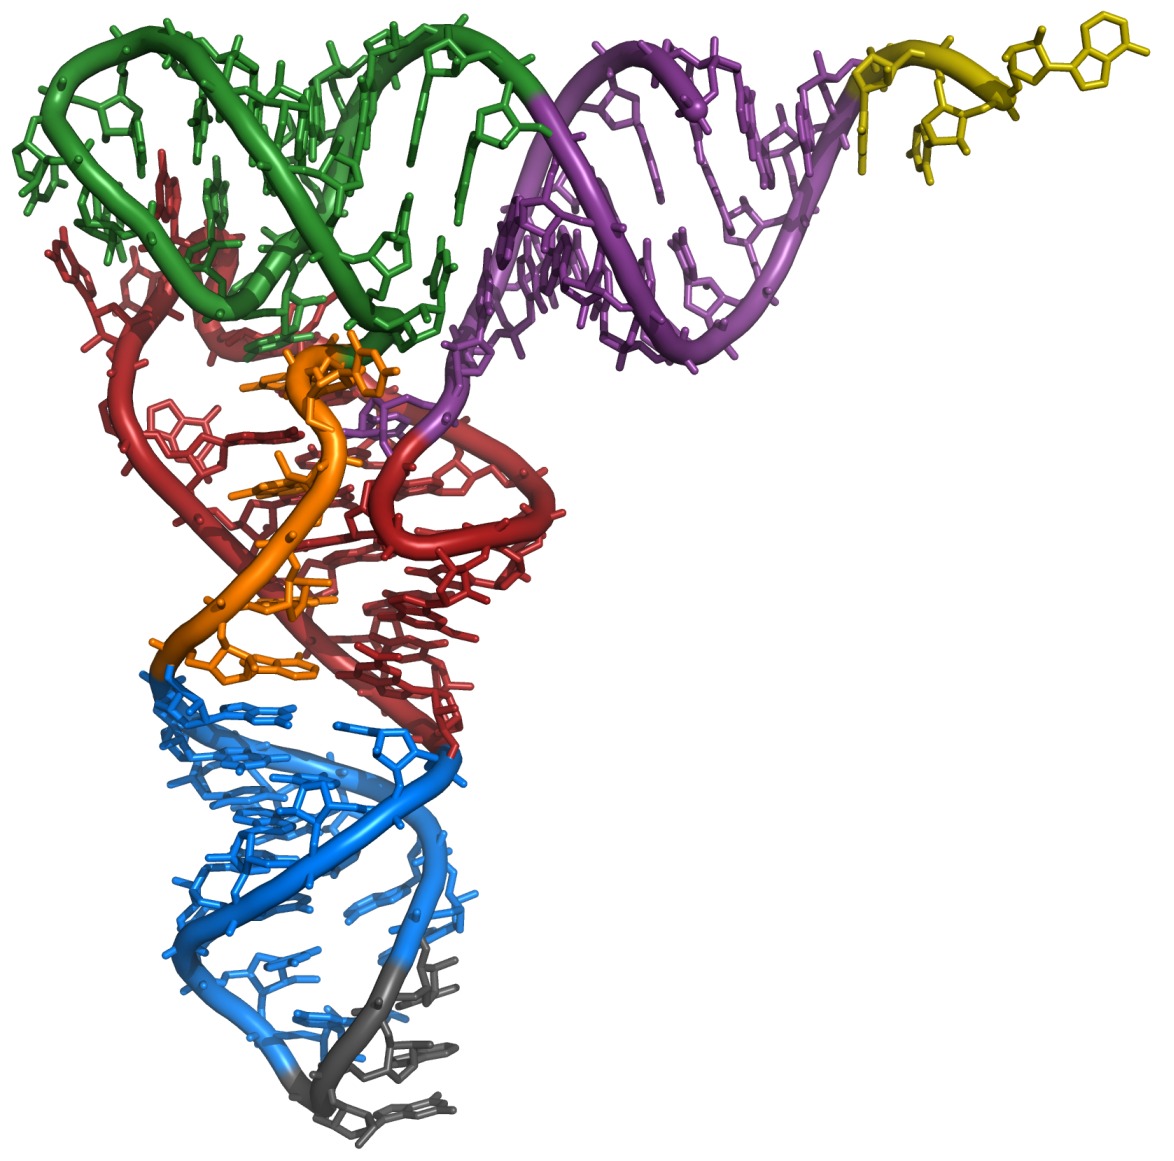
\includegraphics[width=1\linewidth]{../res/images/tertiary.png}
	Tertiary structure of tRNA. The CCA-tail is in yellow, acceptor stem in purple, variable loop in orange, D-arm in red, the anticodon arm in blue with anticodon in black, and T-arm in green (Taken from Wikipedia)}

Each codon represents a particular amino acid, and a specific tRNA recognizes each codon. The tRNA molecule has a distinctive folded structure with three hairpin loops that form the shape of a three-leafed clover. One of these hairpin loops contains an anticodon sequence, which can recognize and decode an mRNA codon. Each tRNA has its corresponding amino acid attached to its end. When a tRNA recognizes and binds to its corresponding codon in the ribosome, the tRNA transfers the appropriate amino acid to the end of the growing amino acid chain. Then the tRNAs and ribosomes decode the mRNA molecule until the entire sequence is translated into a protein (The tertiary structure of a tRNA is shown on the right side of the page). Such studies suggest that RNAs are the actual catalysts of protein synthesis even though proteins remain the common catalysts of various chemical reactions occurring in the cell. This also implies that proteins and RNAs can function as efficient catalysts. 


Apart from being central to the protein machinery, ncRNAs regulate various biological functions in transcriptional interference, telomere maintenance, epigenetic changes, imprinting, post-transcriptional, translational control, structural organization, cell differentiation and development \cite{fatica2014long,santosh2015non}. The ncRNAs are often classified based on their biological functions. Although many recent transcriptomic and bioinformatic studies suggested thousands of ncRNAs with their functional importance, the total number of ncRNAs encoded in the human genome still remains unknown. More recently, newly identified ncRNAs have not been validated by their function; it could be possible that most of them are non-functional. Some experiments \textit{in vitro} evolution have shown that RNA molecules can catalyze a variety of chemical reactions relevant to biological processes such as RNA replication, nucleotide synthesis, thymidylate synthesis, lipid synthesis, and sugar metabolism \cite{robertson1990selection,ellington2009evolutionary}. 

ncRNAs can also be classified based on their lengths formed post-transcriptionally. We often distinguish two main classes of critical biological functions: the short non-coding RNAs (sncRNAs with length $<30nt$) and the long non-coding RNAs (lncRNAs with length $>200nt$). The length limit is often because of the practical considerations, including separating RNAs in standard experimental protocols. The function of lncRNAs includes a role in higher-order chromosomal dynamics, telomere biology, and subcellular structural organization \cite{bergmann2014long,cusanelli2014telomeric}. Some lncRNAs play key regulatory and functional roles in the gene expression program of the cell. One of the vital functions is to act as ribozymes. Examples of naturally occurring ribozymes include group I and group II introns---RNase P and the hammerhead. The group I and group II introns are usually $200-600$nt long, catalyzing RNA splicing. Many sncRNAs also contribute to the realization of similar biological functions. For example, small interfering RNAs contribute to gene regulation, transposon control and vital defence. MicroRNAs participate in the post-transcriptional gene regulation, microRNA-offset RNAs (moRNAs), PIWI-interacting RNAs (piRNAs) and promoter-associated RNAs (PARs) contribute to the gene regulation. More recently,  many discoveries revealed several non-coding RNAs implicated in cancer growth and MCL-1 expression regulation \cite{wang2021circpvt1, santosh2015non}. Those examples include ncRNAs from different classes, miRNAs, snoRNA and T-UCR, all associated with a specific disease \cite{santosh2015non,esteller2011non}. There are also several classes of ncRNAs such as Aptamers and riboswitches that have also been observed in nature. Aptamers are ncRNAs that can bind to other specified targets, whose nature is highly diverse. They range from small molecules to larger molecules. In some contexts, aptamers are termed riboswitches; for example, when their function is to sense the presence of an associated metabolite to cause a specific cis-reaction and/or cis-regulation of subordinated functional pathways \cite{winkler2003genetic}

\section{ncRNA and recent advancements in biotechnology}

Most of the previously mentioned functions of ncRNAs are identified using gene targeting techniques, a well-known technique used to investigate protein functions [ref 155].  With the recent advancements in genome engineering, a method such as Clustered Regularly Interspaced Short Palindromic Repeats (CRISPR) has been employed to tag lncRNAs, allowing to capture specific RNA-protein complexes assembled \textit{in vivo}. The CRISPR \cite{barrangou2007crispr} was first described by Barrangou and his collaborators in 2007 as a distinctive feature of the genomes of most bacteria and archaea and thought to be involved in resistance to bacteriophages. It is an adaptive defence system against viruses and plasmid intrusions. When a successful defence has taken place, the system updates its information about the intruder genetic material. This update will then allows the host of the system to identify its enemy, making robust and durable in the future. The information about the intruder’s genetic material is stored in short repeating stretches of RNA, which can in the case of a new intrusion be incorporated into a carrier protein(CAS). The capacities of the  CRISPR/CAS9 of selectively destroying foreign DNA/RNA and editing the genome was identified by Li et al. \cite{li2016harnessing} and it was turned into methods allowing to selectively alter and edit single genes within genomes. The same technology is also successfully applied to animal cell lines \cite{hwang2013efficient, jinek2013rna, wang2013one} and industrial plants \cite{svitashev2015targeted,li2015cas9}. 

Another method of SELEX (Systematic Evolution of Ligands by EXponential Enrichmen) \cite{tuerk1990systematic} introduced by Tuerk in the early 1990 offers the possibility of enriching stretches of RNA, that can bind towards a certain target. The method relies on mechanisms usually ascribed to the process of evolution, that is, variation, selection, and replication. A pool of RNAs that are completely randomized at specific positions is subjected to selection for binding, in this case to gp43 on nitrocellulose filters. The selected RNAs are amplified as double-stranded DNA competent for subsequent in vitro transcription. This newly transcribed RNA is enriched for better binding sequences and is then subjected to selection to begin the next cycle. Multiple rounds of enrichment result in the exponential in the crease of the best binding ligands until they dominate the population of sequences. In its application SELEX has given raise to multiple synthetic aptamers with different targets. They have been subject to further extension towards inclusion into regulative RNA entities.

\section{Biochemistry of RNA molecules}\label{sec:rna_biochemical}
%\reversemarginpar
\graffito{
	\hspace*{-1cm}
	\scalebox{0.95}{
		
		\chemname[1cm]{\chemfig{
				-[,1.202,,,line width=3.5pt, shorten <=-.05pt, shorten >=-.05pt](-[:-90,,,,line width=1.5pt, shorten >=.5pt]OH)% 2
				>[:44.6,0.521](-[:90, 3.3]{\textcolor{blue}{Nucleobase}})
				-[:167]\chembelow[35pt]{O}{Ribose}
				-[:193,0.998]
				(
				-[:90](-[,0.1,,,draw=none]\chemabove[1ex]{}{\textcolor{gray}{5'}})
				-[::90,1.,,,red](-[::0,,,,red]\color{red}{P}(-[2,,,,red]\color{red}{O^{-}})(-[4,1.3,,,red]\color{red}{O^{-}})(=[6,,,,red]\chembelow{\color{red}{O}}{\textcolor{red}{Phosphate}}))
				)
				(
				<[:315.6,0.522](-[:-90,,,,line width=1.5pt, shorten >=.5pt]OH)(-[::-150,0.4,,,draw=none]\chembelow[1ex]{}{\textcolor{gray}{3'}})
				)
		}	}{Structure of an RNA nucleotide}
	}
\vspace*{6cm}\\
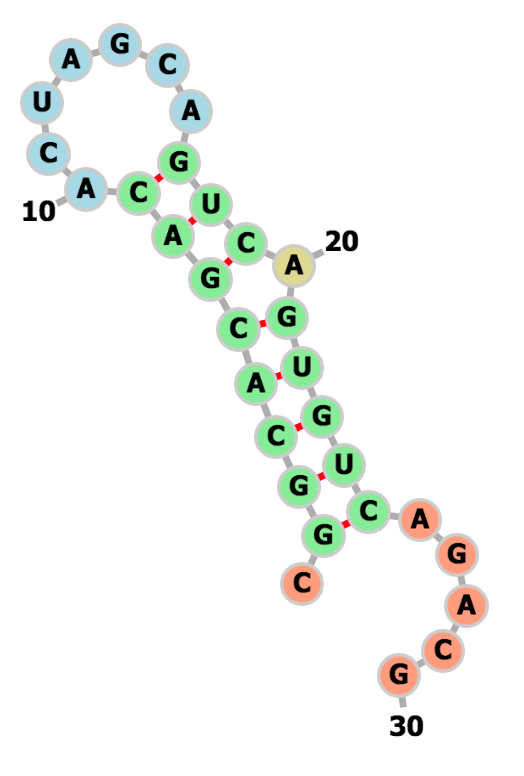
\includegraphics[width=1\linewidth]{../res/images/mfe.png}
An example of secondary structure with a MFE of $8.5$kcal.$mol^{-1}$ (Produced using \texttt{RNAfold} from the \texttt{ViennaRNA} package)
}
RNAs are synthesized from DNAs through a process often termed transcription. The transcription process occurs in the cell's nucleus, and RNA polymerases perform it. Depending on the type of cells, there are many (or one) types of RNA polymerase responsible for synthesizing a specific type of RNA. An RNA polymerase uses the 3’-5' DNA template strand to synthesize a 5’-3' RNA strand with complementary nucleotides during transcription. Similar to DNAs, nucleotides constitute the basis of  RNA molecules, and each nucleotide consists of a phosphate residue, a pentose sugar and a nucleobase. Similar to DNA, we also find four different nucleotides in RNA, distinguished by the nucleobase with only one exception; the Uracil (U), which replaces Thymine in DNA. Figure \ref{fig:nucleotide} depicts the chemical structure of each of the four different nucleobases found in RNA. Chemically, a nucleotide is a nucleoside which has a (mono, di, trip) phosphate residue bound to its 5'-carbon atom. The typical chemical structure of a nucleotide is depicted on the right side of the page. By convention, the carbon atoms of the pentose sugar in nucleotides are numbered with primes.

\begin{figure}
	\begin{minipage}[b]{.5\linewidth}
		\centering
		\subfloat[Adenosine 5'􏱈-monophosphate]{
			\label{fig:adenine}{
				\scalebox{0.9}{
					\chemfig{
						-[,1.202,,,line width=3.5pt](-[:-90,,,,line width=1.5pt]OH)% 2
						>[:44.6,0.521](-[:90] \color{blue}{N}*5(-[,,,,blue]*6(-[,,,,blue]\color{blue}{N}=[,,,,blue]-[,,,,blue]\color{blue}{N}=[,,,,blue](-[:90,,,,blue]\color{blue}{NH_2})-[,,,,blue]-[,,,,blue])=[,,,,blue]-[,,,,blue]\color{blue}{N}=[,,,,blue]-[,,,,blue]))
						-[:167]O
						-[:193,0.998]
						(
						-[:90](-[,0.1,,,draw=none]\chemabove[1ex]{}{\textcolor{gray}{5'}})
						-[::90]O(-[::0]P(-[2]O^{-})(-[4]O^{-})(=[6]O))
						)
						(
						<[:315.6,0.522](-[:-90,,,,line width=0.5pt]OH)(-[::-150,0.4,,,draw=none]\chembelow[1ex]{}{\textcolor{gray}{3'}})
						)
					}	
				}	
		}}\hfill
	\end{minipage}
	\begin{minipage}[b]{.5\linewidth}
		\centering		
		\subfloat[Uridine 5'-monophosphate]{
		\label{fig:uracil}{
			\scalebox{0.9}{\chemfig{
					-[,1.202,,,line width=3.5pt, shorten <=-.05pt, shorten >=-.05pt](-[:-90,,,,line width=1.5pt, shorten >=.5pt]OH)% 2
					>[:44.6,0.521](-[:90] \color{blue}{N}*6(-[,,,,blue](=[,,,,blue]\color{blue}{O})-[,,,,blue]\color{blue}{NH}-[,,,,blue](=[,,,,blue]\color{blue}{O})-[,,,,blue]=[,,,,blue]-[,,,,blue]))
					-[:167]O
					-[:193,0.998]
					(
					-[:90](-[,0.1,,,draw=none]\chemabove[1ex]{}{\textcolor{gray}{5'}})
					-[::90]O(-[::0]P(-[2]O^{-})(-[4]O^{-})(=[6]O))
					)
					(
					<[:315.6,0.522](-[:-90,,,,line width=1.5pt, shorten >=.5pt]OH)(-[::-150,0.4,,,draw=none]\chembelow[1ex]{}{\textcolor{gray}{3'}})
					)
			}}
	}}
	\end{minipage}

	\begin{minipage}[b]{.5\linewidth}
		\centering
		\subfloat[Cytidine 5'􏱈-monophosphate]{
		\label{fig:cytosine}{
		\scalebox{0.9}{	\chemfig{
				-[,1.202,,,line width=3.5pt, shorten <=-.05pt, shorten >=-.05pt](-[:-90,,,,line width=1.5pt, shorten >=.5pt]OH)% 2
				>[:44.6,0.521](-[:90]\color{blue}{N}*6(-[,,,,blue](=[,,,,blue]\color{blue}{O})-[,,,,blue]\color{blue}{N}=[,,,,blue](-[,,,,blue]\color{blue}{NH_2})-[,,,,blue]=[,,,,blue]-[,,,,blue]))
				-[:167]O
				-[:193,0.998]
				(
				-[:90](-[,0.1,,,draw=none]\chemabove[1ex]{}{\textcolor{gray}{5'}})
				-[::90]O(-[::0]P(-[2]O^{-})(-[4]O^{-})(=[6]O))
				)
				(
				<[:315.6,0.522](-[:-90,,,,line width=1.5pt, shorten >=.5pt]OH)(-[::-150,0.4,,,draw=none]\chembelow[1ex]{}{\textcolor{gray}{3'}})
				)
			}
		}
	}}
	\end{minipage}%
	\begin{minipage}[b]{.5\linewidth}
		\centering 
		\subfloat[Guanosine 5'􏱈-monophosphate]{
		\label{fig:guanine}{
			\scalebox{0.9}{	
				\chemfig{
					-[,1.202,,,line width=3.5pt, shorten <=-.05pt, shorten >=-.05pt](-[:-90,,,,line width=1.5pt, shorten >=.5pt]OH)% 2
					>[:44.6,0.521](-[:90] \color{blue}{N}*5(-[,,,,blue]*6(-[,,,,blue]\color{blue}{N}=[,,,,blue](-[,,,,blue]\color{blue}{NH_2})-[,,,,blue]\color{blue}{NH}=[,,,,blue](=[:90,,,,blue]\color{blue}{O})-[,,,,blue]-[,,,,blue])=[,,,,blue]-[,,,,blue]\color{blue}{N}=[,,,,blue]-[,,,,blue]))
					-[:167]O
					-[:193,0.998]
					(
					-[:90](-[,0.1,,,draw=none]\chemabove[1ex]{}{\textcolor{gray}{5'}})
					-[::90]O(-[::0]P(-[2]O^{-})(-[4]O^{-})(=[6]O))
					)
					(
					<[:315.6,0.522](-[:-90,,,,line width=1.5pt, shorten >=.5pt]OH)(-[::-150,0.4,,,draw=none]\chembelow[1ex]{}{\textcolor{gray}{3'}})
					)
				}
			}
			
		}}
	\end{minipage}%
	
	
	\caption{RNA nucleotides. Adenine and guanine belongs into the chemical class of purine molecules and the uracil and thymine in the class of pyrimidines}\label{fig:nucleotide}
\end{figure}
RNA molecules are simply represented as a list of nucleobase characters, and their functions often depend on their complex multidimensional structures. The 5'-3' phosphodiester bonds attach the different nucleotides composing the RNA molecule between ribose to form the primary structure of RNA. The direction of the chain is conventionally designed as 5' to 3' (i.e. from 5'-phosphate of the first sugar backbone to the 3'-hydroxyl of the last sugar in the sequence). The process in which RNA sequences are mapped to their corresponding structures is called RNA folding. In nature, this process is thought to be hierarchical \cite{brion1997hierarchy,tinoco1999rna}. Nucleotides form a chain given their sequence of bases (primary structure); RNAs fold into secondary structures, such as stem-loops and helices, before folding into higher-level (tertiary and quaternary) structures. Our work is restricted here to the secondary level of RNA structures.

In contrast to the RNA primary structure, the secondary structure consists of a list of nucleobase pairs, and the base pairs are formed via hydrogen bonds between the bases. Different interactions are possible between the bases depending on the structure level considered. At the secondary level, we have the Watson-Crick (or canonical) pairs \cite{seeman1976rna, rosenberg1976rna} (A-U and G-C), the Wobble (or non-canonical) (G-U) pairs that occur with reduced frequency. Figure \ref{fig:basepairing} shows the chemical base pairs for the Watson-Crick and Wobble interactions. 

\graffito{
	\vspace*{-3cm}\\
	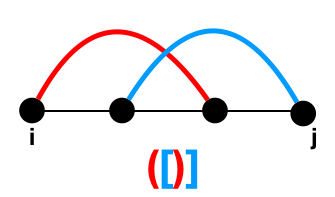
\includegraphics[width=1\linewidth]{../res/images/Hpk.png}
	Hairpin pseudoknot (H-type).
	
	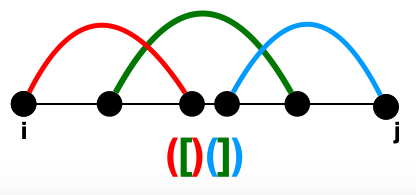
\includegraphics[width=1\linewidth]{../res/images/Kissingpk.png}
	Kissing hairpin pseudoknot (K-type). 
	
	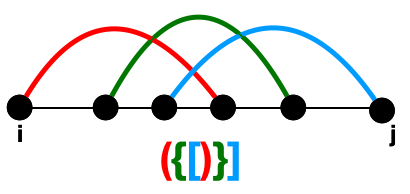
\includegraphics[width=1\linewidth]{../res/images/cHpk.png}
	Complex hairpin pseudoknot (CH-type).}


\begin{figure}
	\hspace*{-5cm}
	\begin{minipage}[b]{0.7 \linewidth}
		\centering
		\subfloat[Adenine-Uracil Interaction]{
			\chemfig{
				R-[::42] N*5(
				%(-H)
				-(*6(
				-N=-N?[h1]
				=(-N([::60]-H)([::-60]-H?[h0]))-=
				))
				--N=-
				)
				*5(-[,,,,draw=none](*6(-[,,,,draw=none]-[,,,,draw=none]-[,,,,draw=none](-[,,,,draw=none]))))
				\phantom{A}-[,1.95,,,draw=none]
				-[::-60,2,,,draw=none]-[,2,,,draw=none]-[::120,,,,draw=none]
				N*6(%(-H)
				-=-(=O?[h0,,{dash pattern=on 1pt off 4pt}, {line width=1.5pt}, gray])-N(-H?[h1,,{dash pattern=on 1pt off 4pt}, {line width=1.5pt}, gray])-(=O?[h2,,{dash pattern=on 1pt off 4pt}, {line width=1.5pt}, gray])-)
				-[::180]R
			}
	
		}
	\end{minipage}%
	%\hspace*{4cm}
	\begin{minipage}[b]{0.7 \linewidth}
		\centering
		\subfloat[Guanine-Cytosine Interaction]{
			\chemfig{
				R-[::42]	N*5(
				%(-H)
				-(*6(
				-N=(-{NH_2})
				-N(-H?[h2])
				-(=O?[h1])-=
				))
				--N=-
				)
				*5(-[,,,,draw=none](*6(-[,,,,draw=none]-[,,,,draw=none]-[,,,,draw=none](-[,,,,draw=none]))))
				\phantom{A}-[,1.95,,,draw=none]
				-[::-60,2,,,draw=none]-[,2,,,draw=none]-[::120,,,,draw=none]
				*6()
				N*6(%(-H)
				-=-(-N([::60]-H?[h1,,{dash pattern=on 1pt off 4pt}, {line width=1.5pt}, gray])([::-60]-H))=N?[h2,,{dash pattern=on 1pt off 4pt}, {line width=1.5pt}, gray]-(=O?[h3,,{dash pattern=on 1pt off 4pt}, {line width=1.5pt}, gray])-)
				-[::180]R
		}
	}
	
	\end{minipage}%
	\vspace*{0.3cm}
	\begin{minipage}[b]{0.7 \linewidth}
		\centering
		\subfloat[Guanine-Uracil Interaction]{
		\chemfig{
			R-[::42]	N*5(
			%(-H)
			-(*6(
			-N=(-{NH_2})
			-N(-H?[h2])
			-(=O?[h1])-=
			))
			--N=-
			)
			*5(-[,,,,draw=none](*6(-[,,,,draw=none]-[,,,,draw=none]-[,,,,draw=none]-[,,,,draw=none](-[,,,,draw=none]))))
			\phantom{A}-[,2.95,,,draw=none]
			-[::-60,2,,,draw=none]-[,2,,,draw=none]-[::120,,,,draw=none]
			N*6(%(-H)
			-=-(=O?[h0,,{dash pattern=on 1pt off 4pt}, {line width=1.5pt}, gray])-N(-H?[h1,,{dash pattern=on 1pt off 4pt}, {line width=1.5pt}, gray])-(=O?[h2,,{dash pattern=on 1pt off 4pt}, {line width=1.5pt}, gray])-)
			-[::180]R
		}
		}
	\end{minipage}
	
	\caption{RNA base pair interactions.}\label{fig:basepairing}
\end{figure}


We also find crossing or pseudoknotted interactions in natural RNA that play vital roles in realising biological functions. Pseudoknots occur when two canonical or non-canonical interactions cross each other \cite{beyongWCpairs}. An example of the three type of pseudoknots often find in RNA is depicted on the left side. Even though pseudoknots are often considered the beginning of the interaction between the secondary and tertiary levels of RNA structures, we consider them part of the secondary structure. Therefore, two main secondary structure definitions are considered in this work: a pseudoknot-free one in which only canonical interactions with no crossing pairs are allowed and a second one where canonical interactions with possible crossing pairs are permitted. 
%\begin{figure}
%	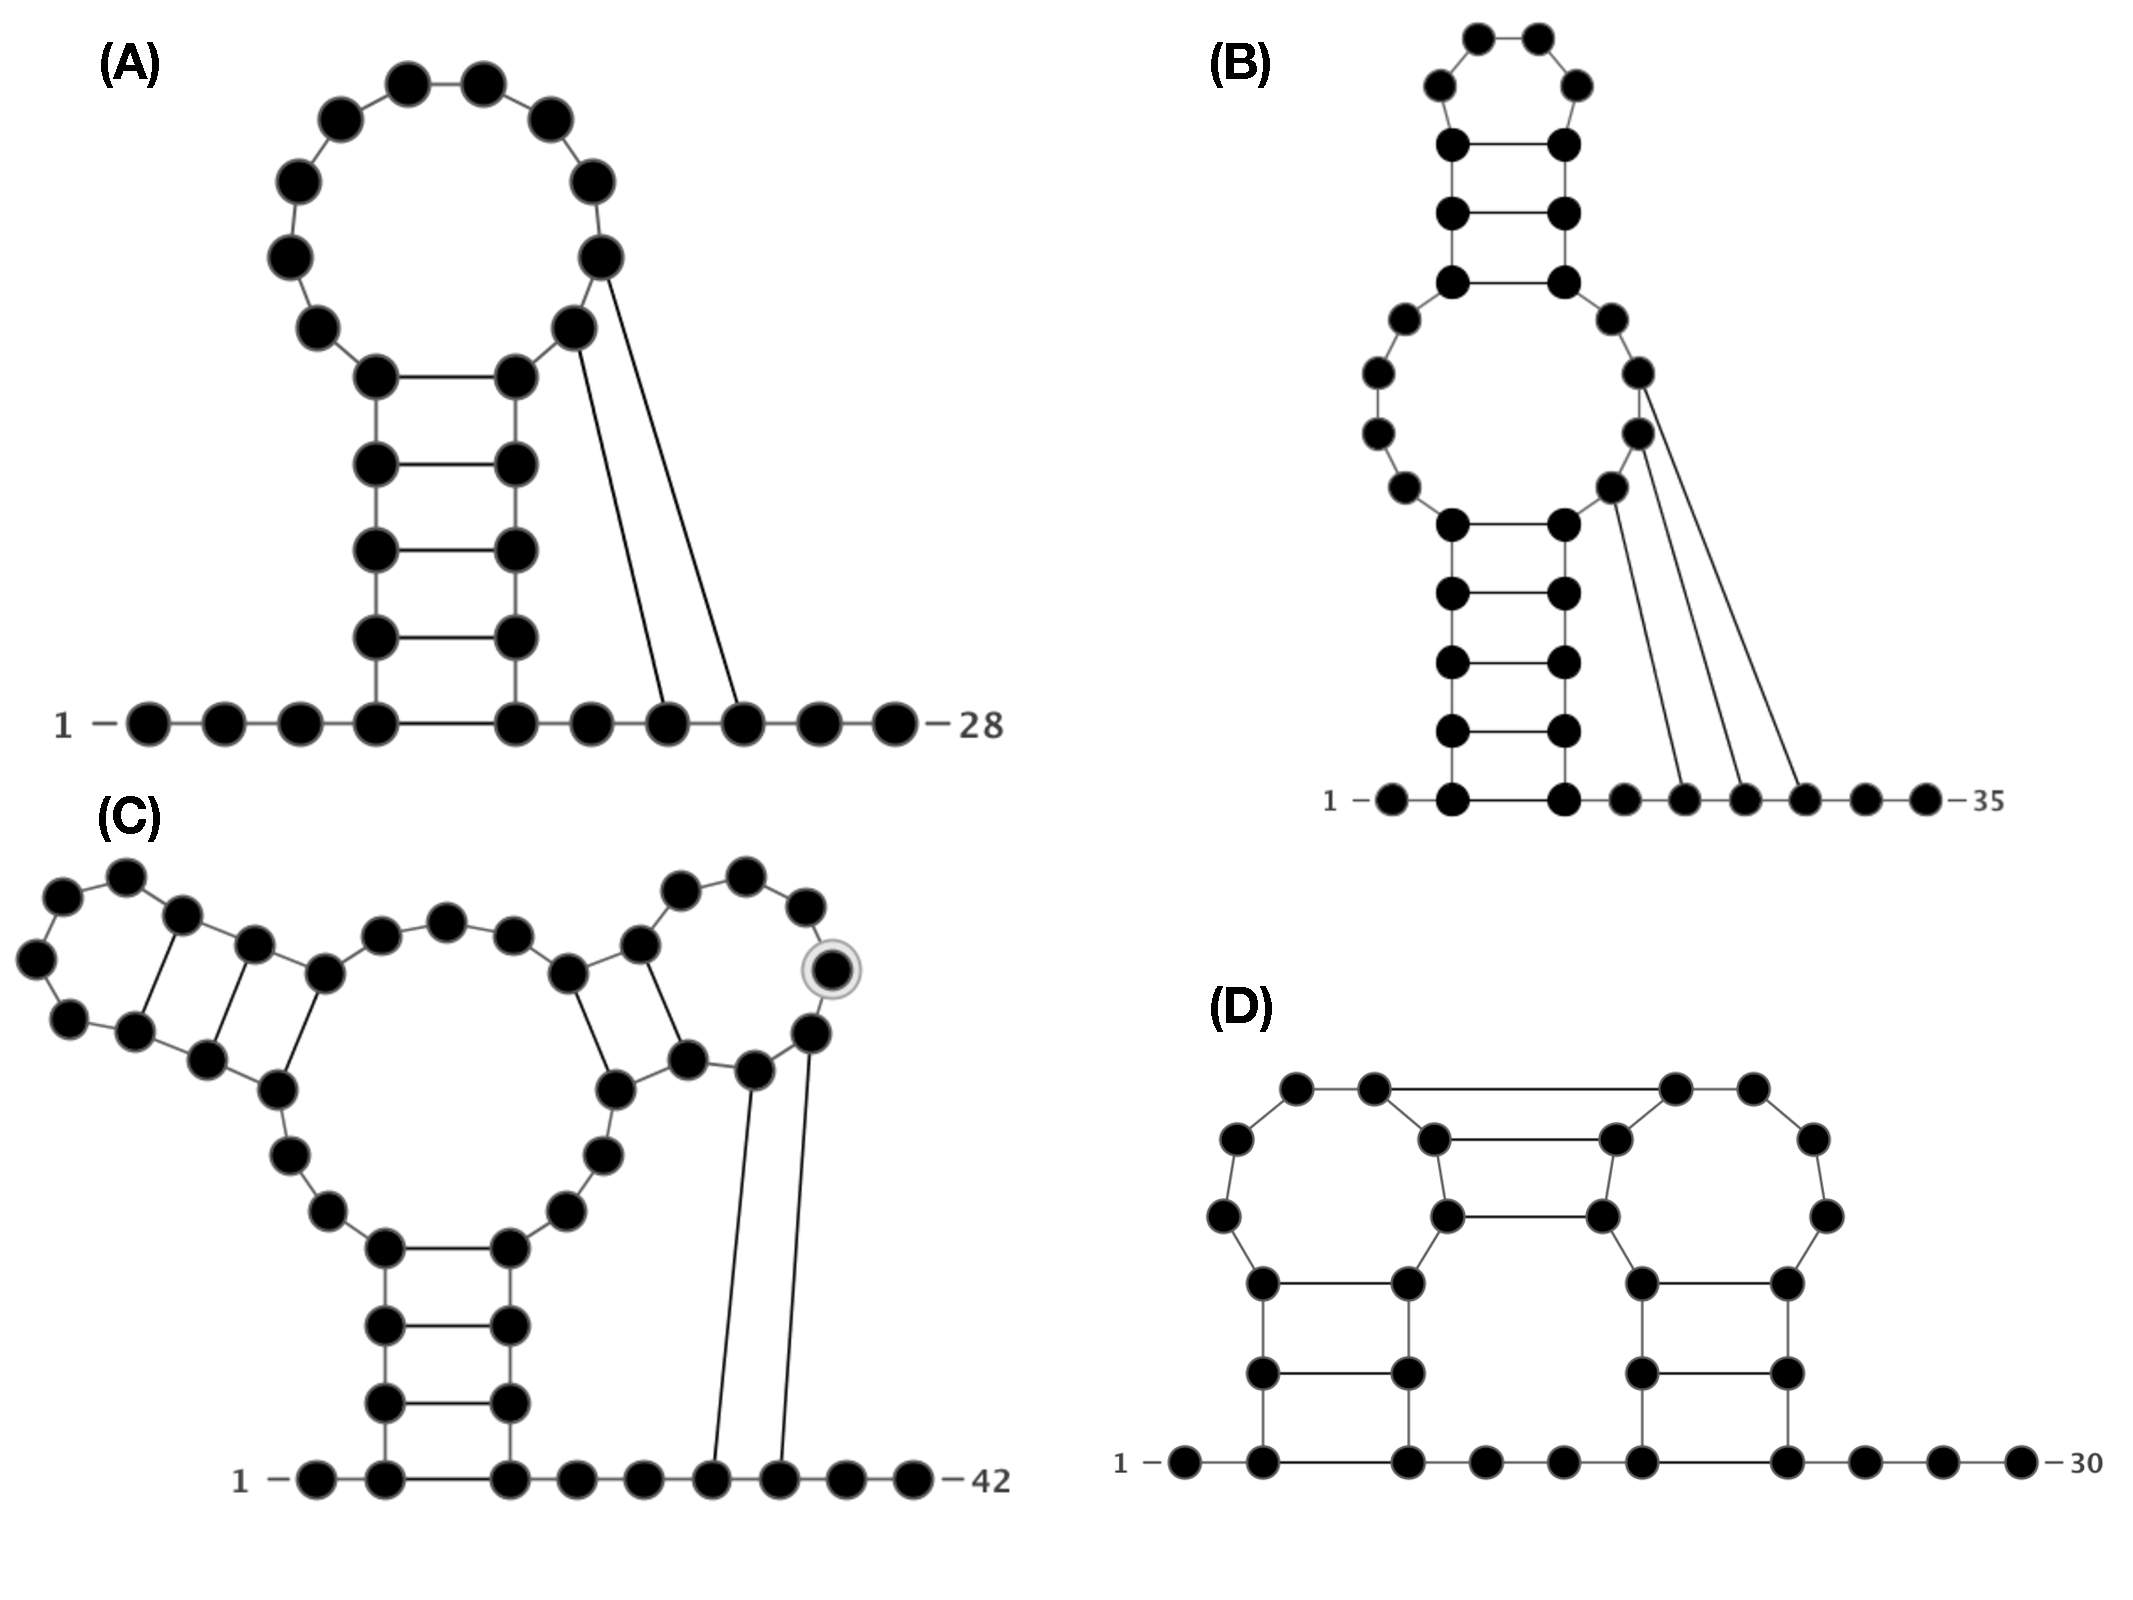
\includegraphics[width=1.0 \linewidth]{../res/images/arnaque/pk_type}
%	\caption{RNA pseudonotted interactions}
%	\label{Fig:pk_type}
%\end{figure}

%\subsection{Biological function of non-coding RNAs}\label{sec:custom}
%Among the number of ncRNAs encoded by the human genomes, most of the ncRNAs have been widely implicated in regulating cellular homeostasis and some are directly involved in epigenetic changes and/or modifications in cells. The ncRNAs are often classified on the basis of their biological functions. Although many recent transcriptomic and bioinformatic studies suggested thousands of ncRNAs with their functional importance, the total number of ncRNAs encoded in the human genome still remains unknown. More recently, newly identified ncRNAs have not been validated by their function, it could be possible that most of them are non-functional. The functional ncRNAs can be classified in to three subsets: (1) the ncRNA implicated in the translation process, (2) the short non-coding RNAs and the (3) the long non-coding RNAs (lncRNAs).

%\subsubsection*{The implication of ncRNAs in the translation process}

%It includes a subset of ncRNAs which is processed in to functionally important RNAs such as transfer RNA(tRNA), ribosomal RNA (rRNA). Transfer ribonucleic acid (tRNA) is a type of RNA molecule that helps decode a messenger RNA (mRNA) sequence into a protein. tRNAs function at specific sites in the ribosome during translation, which is a process that synthesizes a protein from an mRNA molecule. Proteins are built from smaller units called amino acids, which are specified by three-nucleotide mRNA sequences called codons. Each codon represents a particular amino acid, and each codon is recognized by a specific tRNA. The tRNA molecule has a distinctive folded structure with three hairpin loops that form the shape of a three-leafed clover. One of these hairpin loops contains a sequence called the anticodon, which can recognize and decode an mRNA codon. Each tRNA has its corresponding amino acid attached to its end. When a tRNA recognizes and binds to its corresponding codon in the ribosome, the tRNA transfers the appropriate amino acid to the end of the growing amino acid chain. Then the tRNAs and ribosome continue to decode the mRNA molecule until the entire sequence is translated into a protein. ribosomal RNA (rRNA), molecule in cells that forms part of the protein-synthesizing organelle known as a ribosome and that is exported to the cytoplasm to help translate the information in messenger RNA (mRNA) into protein.

%\subsubsection*{The short and long non-coding RNAs}

\section{Bioinformatic definitions.}
In order to computationally study and analyse RNA molecules, a more formal representation of RNAs and bioinformatic definitions are required. We provide in this section formal definitions and concepts that will support the result presented in this thesis.

\paragraph{\textbf{Definition 1}} ( RNA sequence): Let $\phi$ be an RNA sequence of length $L$.  More formally, $\phi$ consists of an ordered sequence of nucleotides that can be represented as:~ \begin{equation}
\phi\ =\ \left(\phi_1,...,\phi_L\right),
\end{equation}
where $\phi_i\in\left\{\text{A},\text{C},\text{G},\text{U}\right\}$ for $i\in \{1\dots L\}$.
\(\phi\)~is often known as the primary structure of RNA.

\paragraph{\textbf{Definition 2} } (RNA pseudoknot-free secondary structure): Given an RNA sequence $\phi \in \left\{\text{A},\text{C},\text{G},\text{U}\right\}^L$, let $\mathcal{P}=\big \{(i,j) \colon i<j \big \}$ be the list of possible pairing positions over the sequence $\phi$. A pseudoknot-free secondary structure $ \mathcal{S}\subset \mathcal{P} $ of such sequence $\phi$ is a list of base pairs  with the following constraints:
\begin{enumerate}
	\item A nucleotide (sequence position) can only belong to a single pair, i.e. $\forall (i,j), (k,l) \in \mathcal{S}$ with $i<k \colon i=k \Rightarrow j=l$.
	\item Paired bases must be separated by at least three
	bases. i.e. \(\forall (i,j) \in \mathcal{S} \Rightarrow \) \(j-i>3\).
	\item There are no pseudoknots, i.e. $ \nexists \left(i,j\right), \left(k,l\right) \in \mathcal{S}$
	~with~\(i<k<j<l\),
	\item The base pairs consist almost exclusively of Watson–Crick ($C–G$ and $A–U$) pairs and Wobble ($G–U$) pairs. i.e. $\forall \left(i,j\right) \in \mathcal{S}\Rightarrow \phi_i\phi_j \in \left\{GC,CG,AU,UA,GU,UG\right\}$,
\end{enumerate}
\paragraph{\textbf{Definition 3} } (Secondary structure representation): A graphical way of representing an RNA secondary structure. Let $\mathcal{S}$ be a secondary structure of an RNA sequence $\phi$ of length $L$. There are several representations of $\mathcal{S}$. 
\begin{itemize}
	\item Dot-bracket (or string) representation: In a this representation, the secondary structure $\mathcal{S}$  is compactly stored in a string $\sigma$ consisting of dots and matching brackets. i.e.  $\sigma$ is a string of length $L$ over the alphabet $\Delta_{\sigma}= \big\{ (,),[,],\{,\},<,>,.\big\}$ where, at each unpaired positions we have a dot '.' at the corresponding string position, and $\forall (i,j) \in \mathcal{S}$, we have an opening bracket at position $\sigma_i$ and a closing bracket at position $\sigma_j$. We denote $\sigma$ the string representation of the structure $\mathcal{S}$. Figure \ref{fig:representation}A shows an example of a string representation.
	\item Planar representation: it is the common way of representing an RNA secondary structure in which $\mathcal{S}$ is presented as a graph with each vertex representing a nucleotide  and an edge connecting consecutive nucleotides and base pairs (See Figure \ref{fig:representation}C). 
	\item Circular (or circle ) representation: similar to planar representation, $\mathcal{S}$  is a graph but drawn in the plane in such a way that all vertices are arranged on a circle, and the edges representing base pairs lie inside the circle. In a pseudoknot-free secondary structure circular representation, the edges do not intersect (See Figure \ref{fig:representation}B).  
	\item Linear representation: In this representation, $\mathcal{S}$  is a graph in which the nucleotides are arranged consecutively in a line and the edges representing base pairs form semi-circle that do not intersect for pseudoknot-free structure (See Figure \ref{fig:representation}D).
	\item Mountain representation: it is mainly used for representing large structures. $\mathcal{S}$  is presented in a two-dimensional graph, in which the $x$-coordinate is the position $i$ of the nucleotide in the sequence $\phi$ and the $y$-coordinate the number $m(i)$ of base pairs that enclose nucleotide $i$.
	\item Tree representation: $\mathcal{S}$  is drawn as a tree in which internal nodes are the base pairing positions, and the leaves are the unpaired positions. The dot-bracket representation is also often considered as a tree represented by a string of parenthesis (base pairs) and dots for the leaf nodes (unpaired nucleotides). 
	\item Shapiro representation: it allows representing the different elements composing $\mathcal{S}$  by single matching brackets, and the components are labelled with H(Hairpin), B(Bulge), I (interior loop), M (multi-loop) and S (stacking loop) \cite{shapiro1990comparing}.
\end{itemize}
Figure \ref{fig:representation} shows some examples of RNA secondary structure representation.
\begin{figure}
	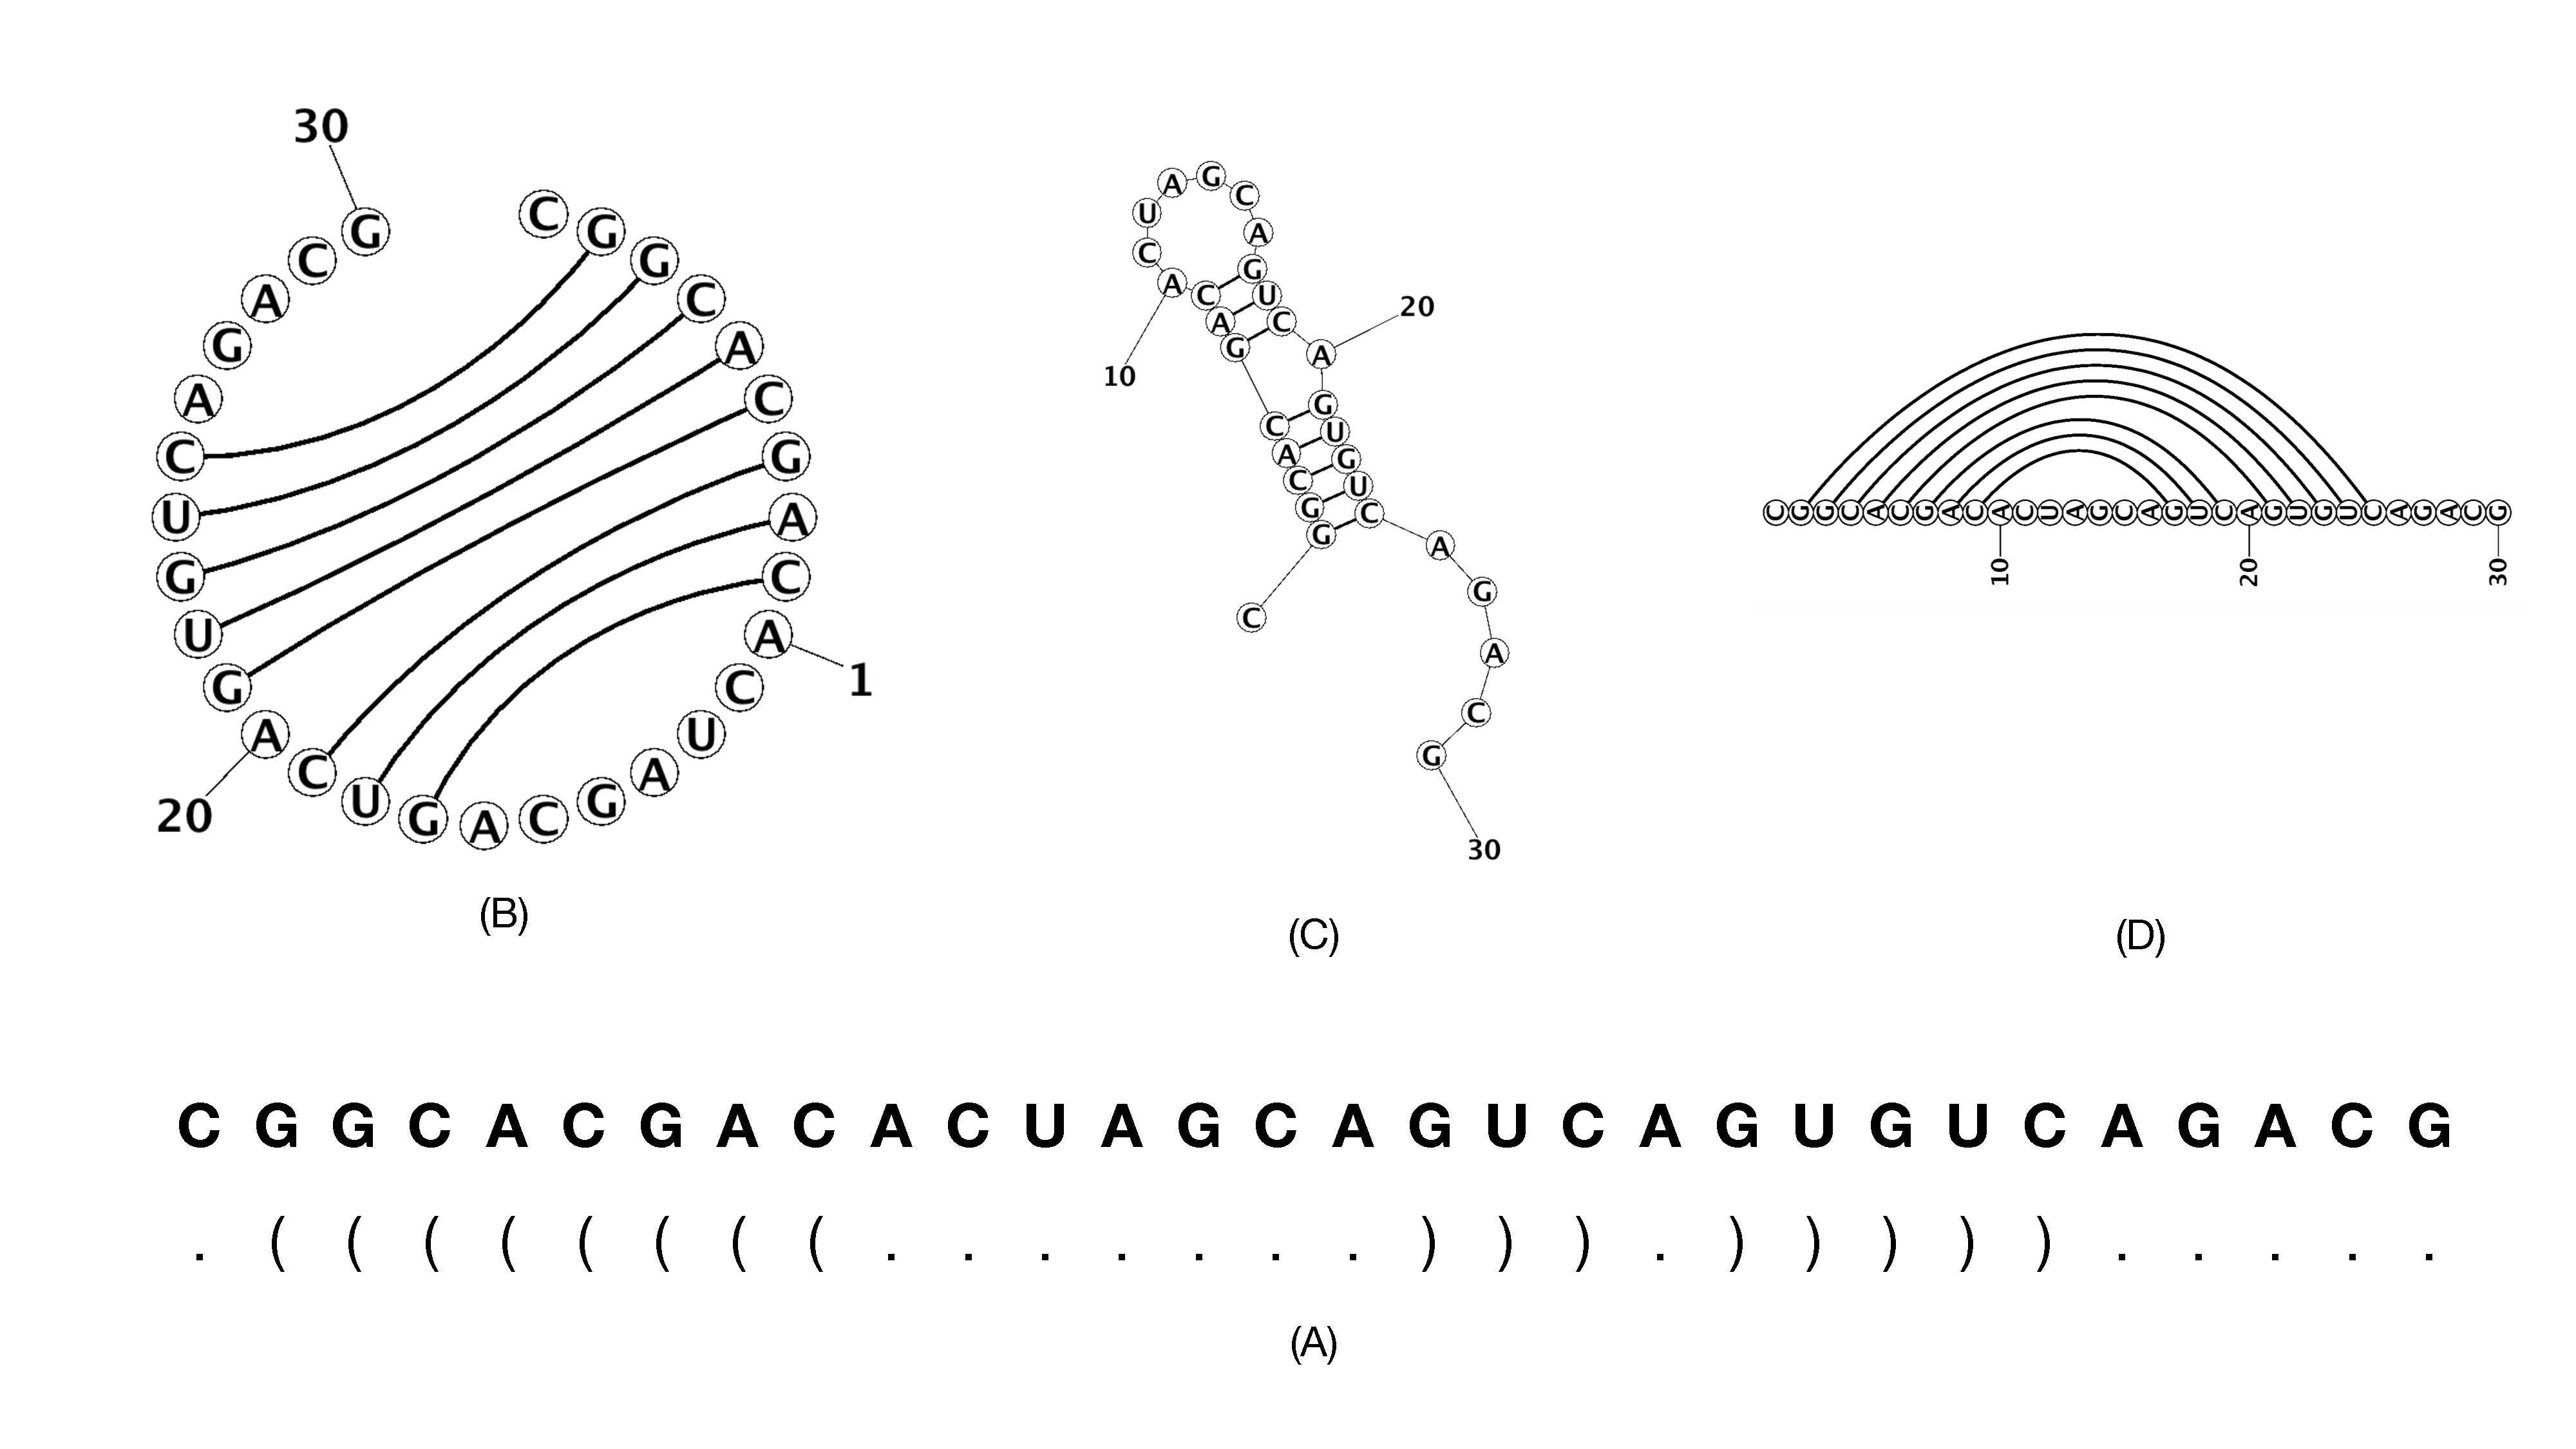
\includegraphics[width=1.0 \linewidth]{../res/images/arnaque/intro/RNA_reps}
	\caption{RNA secondary structure representation}\label{fig:representation}
\end{figure}

\paragraph{\textbf{Definition 4} }(Secondary structure loop):  Given a secondary structure $\mathcal{S}$ over an RNA sequence $\phi$ of length $L$, there exists a unique decomposition of $\mathcal{S}$ into a set of $n$ loops $\mathbb{L}_{\phi, \mathcal{S}}$, where loops are the faces of its planar drawing. Each loop $\mathcal{L} \in \mathbb{L}_{\phi, \mathcal{S}}$ is characterised by its length $l$ (the number of unpaired nucleotides in the loop) and its degree $d$ (the number of base pairs delimiting the loop, including the closing loop pair). 

By definition, $\forall  \mathcal{L} \in \mathbb{L}_{\phi, \mathcal{S}} \Rightarrow \mathcal{L}  = \mathcal{L}_p \cup \mathcal{L}_u$ where $\mathcal{L}_p$ and $\mathcal{L}_u$ denote respectively the set of loop base pairs and the unpaired positions. $\mathcal{L}_p$ contains only one closing loop and the rest are enclosed base pairs. We say $(i,j) \in \mathcal{L}_p$ is a closing pair if and only if $\forall \mathcal{L}_p \ni (i',j') \neq (i,j) \colon i<i'<j'<j$.

\graffito{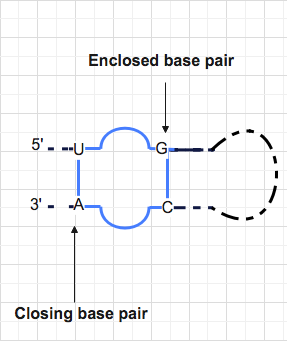
\includegraphics[width=1\linewidth]{../res/images/interior.png}
	An example of closing and enclosed base pairs of an interior loop.
}
\begin{enumerate}
	\item Interior loop: a loop with degree $d=2$ i.e $|\mathcal{L}_p|=2$ and $\mathcal{L}_u \subset \{1,2,\dots L\}\cup \emptyset$.
	\item Stacking pair: an interior loop of length $l=0$ i.e. $|\mathcal{L}_p|=2$ and $\mathcal{L}_u = \emptyset$.
	\item Hairpin Loop: Any loop of degree $d=1$ and length $l \geq 3$.  i.e $|\mathcal{L}_p|=1$ and  $\mathcal{L}_u \neq \emptyset$.
	\item Bulge loop: a special case of interior loop in which there are unpaired bases only on one side. i.e  $\mathcal{L}_p=\{(i_1,j_1), (i_2, j_2)\}$ with $i_1 \neq i_2, j_1\neq j_2$ one of the following assumption holds: 
		\begin{itemize}
			\item If $\exists i'\in \mathcal{L}_u \colon i_1<i'<j_2 \Rightarrow \nexists k'\in \mathcal{L}_u \colon i_2<k'<j_2$ 
			\item If $\exists k'\in \mathcal{L}_u \colon i_2<k'<j_2 \Rightarrow \nexists i'\in \mathcal{L}_u \colon i_1<i'<j_1$ 
		\end{itemize}
	\item Multi-loop: Any loop with degree $d>2$ i.e.  $|\mathcal{L}i_p| \geq 3$  and $\mathcal{L}_u \neq \emptyset$.
	\item Exterior loop: a loop in which all the positions are not interior of any pair i.e. $\mathcal{L}_p=\emptyset$ and $\mathcal{L}_u \neq \emptyset$.
\end{enumerate}

\begin{figure}[H]
	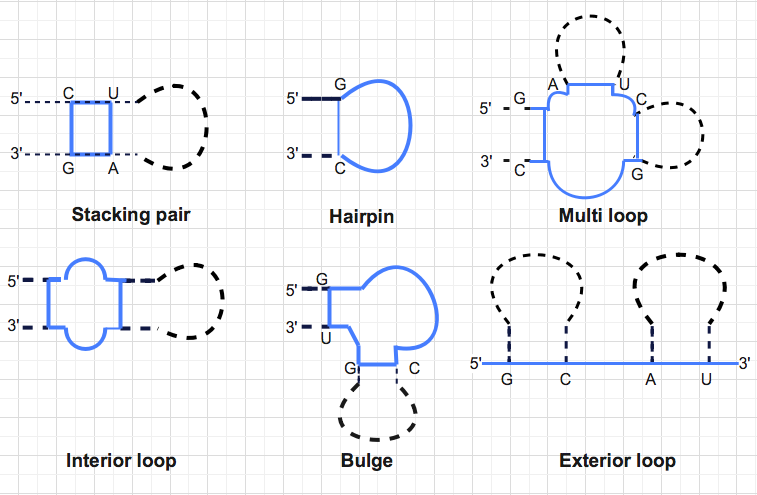
\includegraphics[width=1.0 \linewidth]{../res/images/loops2.png}
	\caption{RNA secondary structure loop decomposition}\label{fig:loops}
\end{figure}

\paragraph{\textbf{Definition 5}} (Free Energy of an RNA secondary structure): Given an RNA sequence $\phi$, its secondary structure $\mathcal{S}$ and its loop set $\mathbb{L}_{\phi, \mathcal{S}}$; the free energy \(\Delta G\) of $\mathcal{S}$ defines its thermodynamic stability. \(\Delta G\) is the free energy difference with respect to the completely unfolded state \cite{tinoco_estimation_1971}. \(\Delta G (\mathcal{S}, \phi)\) is computed using the additivity principle \cite{dill97_addit_princ_bioch}, by summing up its constituent loops free energies.
\begin{equation}
	 \Delta G(\mathcal{S}, \phi) = \sum_{\mathcal{L}\in \mathbb{L}_{\mathcal{S}, \phi}}{ \Delta G(\mathcal{L}) }
\end{equation}
Many models allow for computing the free energies of those constituent loops, but the dominant one is the nearest-neighbor loop energy model \cite{turner09_nndb}. This model associates tabulated free energy values to loop types and nucleotide compositions; the Turner2004 \cite{mathews2004incorporating} is one of the most widely used parameter sets. 

The free energy of each a given loop $\mathcal{L}$ is expressed as
\begin{equation}\label{eq:gibbs}
\Delta G (\mathcal{L}) = \Delta H - T \Delta S \leq 0
\end{equation}
where $\Delta H$ is the (pressure- and volume-dependent) enthalpy change, $T$ the absolute temperature and $\Delta S$ the entropy change. 
The dominant stabilizing effect is attributed to consecutive base pairs (The stacking loops), whereas long unpaired regions enclosed between base pairs have destabilizing effects \cite{fresco_molecular_1960, hofacker_rna_2006}. As a simplified example, the destabilizing free energy contribution $\Delta G(\mathcal{L}_m)$ of a multiloop $\mathcal{L}_m$  as seen in \ref{fig:loops}C is modelled as:
\begin{equation}\label{eq:multi}
\Delta G(\mathcal{L}_m) = \Delta G_\mathrm{init} + b \Delta G_\mathrm{branch} + u \Delta G_\mathrm{unpaired}
\end{equation}
where $b$ is the number of all surrounding base pairs and $u$ the number of base pairs \parencite{dirks_partition_2003}.
%This structure decomposition allows an efficient dynamic programming algorithm that can determine the minimum free energy (MFE) structure of a sequence in the entire structure space. The gold standard for free-energy-based predictions is usually the MFE; however, it represents one structural estimate among many others, such as the maximum expected accuracy (MEA).    

\paragraph{\textbf{Definition 6}}  (Structure Ensemble):  For a given RNA sequence $\phi$,  the set of all pseudoknot-free secondary structures with their corresponding energies is called the structure ensemble $\Sigma_{\phi}$ of $\phi$.  We write: 

$$
\Sigma_{\phi} = \{ \mathcal{S} | \mathcal{S} \text{ is a secondary structure of $\phi$}\}
$$

According to the nearest neighbor energy model, all possible secondary structures of a given RNA sequence do not have the same energy. Since each structure has a unique decomposition, each structure has its own energy but different structures can have the same energy.

\paragraph{\textbf{Definition 7}} (Partition function of RNA): Given the free energy change $\Delta G(\mathcal{S})$ of a structure $\mathcal{S}$, the partition function $Z(\Sigma_{\phi})$ is defined on the Boltzmann ensemble (or structure ensemble) of all possible structures of a given sequence $\phi$ and we write: 

\begin{equation}
	Z(\Sigma_{\phi}) = \sum_{\mathcal{S} \in \Sigma_{\phi} }{\exp(-\beta \Delta G(\mathcal{S}, \phi))}
\end{equation}

Where, $\beta = (RT)^{-1}$ with $R$ the ideal gas constant, and $T$ the temperature.

\paragraph{\textbf{Definition 8}} (Secondary structure probability):
Given an RNA sequence $\phi$ and its structural ensemble $\Sigma_{\phi}$, 
how probable is an RNA secondary structure $\mathcal{S} \in \Sigma_{\phi}$ for the sequence $\phi$? Given the free energy change $\Delta G(\mathcal{S})$ of a structure $\mathcal{S}$, the boltzmann distribution describes the structure's probability at constant temperature $T$ among all other possible structure of the same sequence $\phi$.
The probability $p(\mathcal{S}| \phi)$ depends on the free energy $\Delta G(\mathcal{S})$, the lower the more probable. We write: 

\begin{equation}
	p(\mathcal{S}| \phi)= \frac{\exp(-\beta \Delta G(\mathcal{S}, \phi))}{Z}
\end{equation}

where, $Z$ is the partition function and $\beta = (RT)^{-1}$ the thermal constant. 


\paragraph{\textbf{Definition 9}} (MFE secondary structure): 
To predict biologically relevant structures, most computational methods search for structures that minimize the free energy. For a given sequence $\phi$, let~\(\Sigma_{\phi}\) be the secondary structure ensemble of~\(\phi\). The minimum free energy structure $\mathcal{S}_{MFE}$ is the structure with the lowest probability $p(\mathcal{S}|\phi)$ i.e. the  most stable conformation in the thermodynamic equilibrium. We write:

\begin{equation}
\mathcal{S}^{MFE}(\phi) = \arg \min_{\mathcal{S} \in \Sigma_{\phi}} \Delta G(\mathcal{S}, \phi) 
\end{equation}

\paragraph{\textbf{Definition 10}}(Base pair probability): Let $\phi=(\phi_i)_{1\leq i \leq L} $ be an RNA sequence. The base pair probability matrix $\mathbf{P}(\phi)$ quantifies the equilibrium structural features of the ensemble $\Sigma_{\phi}$, with entries $P_{i,j}(\phi) \in [ 0,1]$ defines as follows: 

\begin{equation}
	P_{i,j}(\phi) = \sum_{\mathcal{S} \in \Sigma_{\phi}}{p(\mathcal{S}|\phi)S_{i,j}(\mathcal{S})}
\end{equation} 

$P_{i,j}(\phi)$ corresponds to the probability that base pair $i.j$ forms at the equilibrium. 
\(\mathbf{S}(\mathcal{S})\) is the structure matrix with entries \(S_{i,j} \in  \{ 0, 1\}\). If the structure \(\mathcal{S}\) contains pair~ $(i ,j)$, then \(S_{i,j}(\mathcal{S}) = 1\)~otherwise \(S_{i,j}(\mathcal{S}) = 0\).

\paragraph{\textbf{Definition 11}} (Neutral set of RNA sequences): 
The size of the RNA structural ensemble has been analytically computed through tools developed by Stein and Waterman \cite{stein1979some}, and it yields an upper bound of~\(S_L\approx1.48\times L^{-\frac{3}{2}}1.85^L\) structure vis-a-vis~\(4^L\) sequences.
Compared to the total number of sequences, the number of structures is much smaller, which means there is indeed a high possibility that many sequences fold into the same MFE secondary structure. In case that happens, we call the set of those sequences a neutral set. 

\paragraph{\textbf{Definition 12}} (Neutral Network): it is a graph in which vertices are neutral sequences and, two vertices are adjacent when they differ by a single nucleotide.
%\reversemarginpar
%\graffito{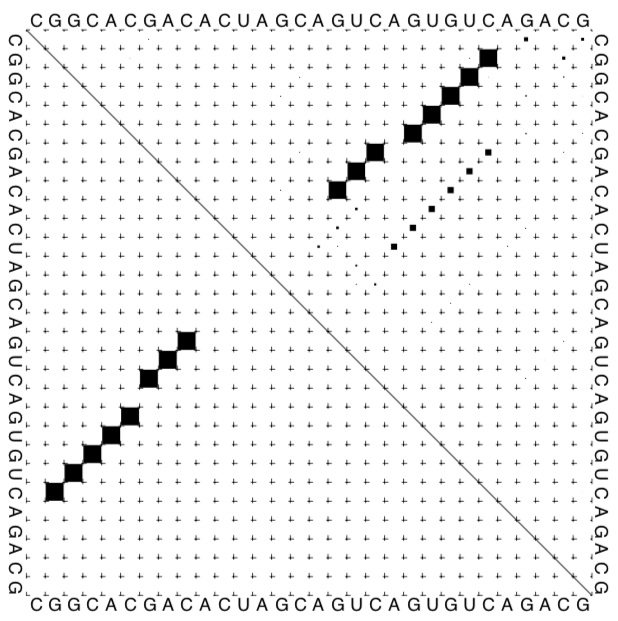
\includegraphics[width=1\linewidth]{../res/images/prob.png}
%	An example of the base pair matrix probabilities.}
\paragraph{\textbf{Definition 13}}  The positive predictive value (PPV):  it measures the fraction of correct base pairs in the predicted structure and it is defined as follows: 

\begin{equation}
	PPV = \frac{TP}{TP + FP}
\end{equation}

where TP and FP stand respectively for the number of correctly predicted base pairs (true positives), and the number of wrongly predicted base pairs (false positives). 

\paragraph{\textbf{Definition 14}} (Sensitivity): it measures the fraction of
base pairs in the accepted structure that are predicted.
\begin{equation}
\text{Sensitivity} = \frac{TP}{TP+FN}
\end{equation}
where FN stands for the number of base pairs not detected (false
negatives).

\paragraph{\textbf{Definition 15}} (Hamming Distance):  Let $\sigma_1$ and $\sigma_2$ be two secondary structures in their string representation. We define the hamming distance between $\sigma_1$ and $\sigma_2$, $d_h(\sigma_1, \sigma_2)$, to be the number of position where $\sigma_1$ and $\sigma_2$ differ.  

\begin{equation}
	d_h(\sigma_1, \sigma_2) = \sum_{i=1}^{L}{S(\sigma_1^i, \sigma_2^i)}
\end{equation}
where, 
$$
S(\sigma_1^i, \sigma_2^j) =
\begin{cases}
1 & \text{if $\sigma_1^i \neq \sigma_2^j)$ } \\
0 & \text{otherwise}
\end{cases}
$$
\paragraph{\textbf{Definition 16}} (Ensemble defect (ED)) \citep{zadeh2011nucleic}: Given an RNA sequence $\phi$ of length $L$, the ensemble defect $\mathcal{D}_E$ is the expected base pair distance between a target structure $\mathcal{S}^*$  and a random structure generated with respect to the Boltzmann probability distribution. It is defined as follows: 

\begin{equation}
\label{ed}
\begin{split}
\mathcal{D}_E(\phi, \mathcal{S}^*) 
&= \sum_{\mathcal{S} \in \Sigma_{\phi}}{p(\mathcal{S}|\phi)d_{bp}(\mathcal{S},\mathcal{S}^*)}\\
&= L - \sum_{1<i,j<L} P_{i,j}(\phi)S_{i,j}(\mathcal{S}^*)
\end{split}
\end{equation}

where~\(P_{i,j}\)~is the base pair probability matrix entrances, $d_{bp} ((\mathcal{S},\mathcal{S}^*))$ is the base pair distance between two structures, and \(\mathbf{S}(\mathcal{S})\) is the structure matrix with entries \(S_{i,j} \in  \{ 0, 1\}\). If the structure \(\mathcal{S}\) contains pair~ $(i ,j)$, then \(S_{i,j}(\mathcal{S}) = 1\)~otherwise \(S_{i,j}(\mathcal{S}) = 0\).

\paragraph{\textbf{Definition 17} } Normalized Energy Distance (NED): the difference between
the energy of a given sequence~\(\phi\)~evaluated to fold into a target structure $\mathcal{S}^*$ and the minimum free energy of the sequence in its structural ensemble~\(\Sigma_{\phi}\).~ The value is normalized over all the sequences in a given population $P$.  


\begin{equation}
\label{ned}
\mathcal{N}_E (\phi, \mathcal{S}^*) = [1-\Delta \hat{E}(\mathcal{S}^*,\phi)]^q \text{   } \forall q>1
\end{equation}
where,
\begin{equation}
\Delta \hat{E}(\mathcal{S}^*, \phi) = \frac{\Delta E(\mathcal{S}^*, \phi) }{\sum_{s \in P}{\Delta E(\mathcal{S}^*, s)}}
\end{equation}
and,
\begin{equation}
\Delta E(\mathcal{S}^*,\phi) = \Delta G(\mathcal{S}^*, \phi) - \arg \min_{\mathcal{S} \in \Sigma_{\phi\\
}} \Delta G(\mathcal{S}, \phi)
\end{equation}

%\paragraph{\textbf{Definition 17}} (Fitness landscape) :  A fitness landscape $\mathcal{L}$ results from the combination of three elements: a set of configurations $\mathcal{V}$, a cost or fitness function $f$, and a move operator $\phi$ that induces a topology on the set of configurations. We write: 

%\begin{equation}
%	\mathcal{L} = (\mathcal{G}_f, f, \phi)
%\end{equation}

%where $\mathcal{G}_f$  is the the landscape underlying the hypergraph whose vertices are the elements from $\mathcal{V}$ labelled with values given by $f$, and whose edges are specified by the move operator $\Phi$.

%The fitness function $f$ assigns to each configuration $g\in G$ a real value taken from an interval $I\in \mathbf{R}$ as follows: 

%$$
%f: \mathcal{V} \rightarrow \mathbf{I}
%$$

\paragraph{\textbf{Definition 18}} (Base pair distance):  Let $\sigma_1$ and $\sigma_2$ be two secondary structures in their string representation.  The base pair distance between $\sigma_1$ and $\sigma_2$ is defined as follows: 
\begin{equation}
	d_{bp}(\sigma_1, \sigma_2 )= \sum_{i,j} A_{i,j}[\sigma_1] + A_{i,j}[\sigma_2] + 2\times A_{i,j}[\sigma_1] A_{i,j}[\sigma_2],
\end{equation}
where, 
$$
A_{i,j}[\sigma] =
\begin{cases}
1 & \text{if $(i,j)$ is a base pair in $\sigma$ } \\
0 & \text{otherwise}
\end{cases}
$$

%\paragraph{\textbf{Definition 18}} (Local minima): 

%\paragraph{\textbf{Definition 19}} (Global minima): 

%\paragraph{\textbf{Definition 20}} (Lévy Flights): 

%\paragraph{\textbf{Definition 21} }(Local search): 

\paragraph{\textbf{Definition 19}} (Mutation mode): 
Let $\phi, \phi' \in \left\{ \text{A}, \text{C}, \text{G}, \text{U} \right\}^L$, be  two RNA sequences. $\phi'$ is said to be an $n$-point mutation of $\phi$ if it differs from $\phi$ at $n$ nucleotides; i.e. $d_h(\phi, \phi')=n$ where $d_h(.,.)$ is the hamming distance on $\left\{ \text{A}, \text{C}, \text{G}, \text{U} \right\}^L$. 

A mutation mode is a random variable $U$ taking values in $\{1,...,L\}$. $P(U=n)$ is defined as the probability that, exactly $n$ nucleotides, selected uniformly at random undergo point mutation during a mutation event. $U$ can generally be any probability distribution.

\section{Conclusion and outline of the thesis}

This introductory chapter presents nucleic acids in general and, in particular, a description of RNA and its chemical, biological, and algorithmic definitions. Those concepts with biological motivations constitute the basis of the thesis. 

The thesis is organized into five chapters. The two first chapters are grouped into a first result part which only concerns the RNA folding. In this first result part, the first chapter provides a brief literature review on the existing computational methods for RNA folding and the second one aim to present our proposed folding tool called \texttt{RAFFT}. Similar to the first part of the result, the second part contains two chapters. The first chapter will briefly introduce the RNA design problem, and in the second one, our proposed algorithm and its performance compared to the existing tools. Finally, the last chapter will present a general conclusion, a discussion on the results obtained and some promising perspectives. 

